\chapter{Higher order AGP as a cost function}\label{chap:7_higher_order_agp}

\epigraph{`Fast' was a word particularly associated with tortoises because they were not it.}{Terry Pratchett, \emph{Pyramids (1989)}}

In Ch.~\ref{chap:5_cd_as_costfunc} we discussed the idea of using the \acrref{AGP} operator and its approximations in order to construct cost functions for the optimisation of Hamiltonian paths in parameter space. There are several reasons why one might expect this to be a good idea: for example, a path in the Hamiltonian parameter space which minimises the \acrref{AGP} norm should, in principle, also minimise the non-adiabatic effects experienced by the system when it is driven along that path. Furthermore, such cost functions should be very efficient to compute once they are written in the correct functional form, giving them an advantage over the fidelity cost function that we used in most examples of Ch.\ref{chap:6_Applications_fidelity}, which suffers from increasing complexity and inefficiency with growing system sizes due to requiring access to the system dynamics along the entire path of the evolution.

In this chapter we will motivate the idea of \acrref{AGP}-based cost functions with numerical results, investigating two types of cost functions presented in Ch.~\ref{chap:5_cd_as_costfunc}: minimisation of absolute integrals of the \acrref{LCD} coefficients and minimisation of their maximal amplitudes. We will do this for three different example systems which we covered in the previous chapter: two-spin annealing in Sec.~\ref{sec:7.1_two_spin_ho}, the Ising spin chain in Sec.~\ref{sec:7.2_ising_ho_lcd} and finally the preparation of maximally entangled GHZ states in systems of frustrated spins in Sec.~\ref{sec:7.3_ghz_ho}. In the last example, we will find a situation where this new approach might not be optimal and discuss the reasons behind why, with the goal of understanding when such an approach is or isn't effective. 

\section{Return to two-spin annealing}\label{sec:7.1_two_spin_ho}

In Sec.~\ref{sec:5.1_2spin_annealing} we investigated the \acrref{COLD} protocol in the case of a two-spin annealing protocol described by the Hamiltonian given by Eq.~\eqref{eq:two_spin_hamiltonian}, where the system starts close to the state $\ket{\uparrow\uparrow}$ and is driven towards a superposition of all the symmetric states. We will return to this simple example in order to illustrate how the integral and maximum amplitude cost functions from Sec.~\ref{chap:5_cd_as_costfunc}, given by Eq.~\eqref{eq:COLD_costfunc_integral} and Eq.~\eqref{eq:COLD_costfunc_maximum} respectively, behave when used to optimise the Hamiltonian path in parameter space for \acrref{COLD}.

In Ch.~\ref{chap:6_Applications_fidelity} we presented the results of optimisation using properties of the final system state as metrics for success. What we wish to demonstrate here is the use of different cost functions in the optimisation of the parameters $c_k$ from Eq.~\eqref{eq:COLD_twospin_controlH}. As discussed in Ch.~\ref{chap:5_cd_as_costfunc}, once we have the \acrref{AGP} or \acrref{LCD} operators expressed as functions of the control Hamiltonian, including a dependence on the control functions $\beta_k \in \betabb$, they can be used to construct cost functions that can be evaluated very efficiently, regardless of the scale or complexity of the driven system. This is important, as while the fidelity cost function $C_{\rm F}$ from Eq.~\eqref{eq:costfunc_fidelity} that we used in the previous chapter is very effective, given that it evaluates exactly how close we are to the goal of the optimisation, its efficiency scales very poorly with increasing system size. After all, having access to the final state fidelity requires a calculation of the complete system dynamics, as well as knowledge of the target state ahead of time. 

In this example, we will use the same control Hamiltonian as the two-spin example from the previous chapter given by Eq.~\eqref{eq:COLD_twospin_controlH} as well as the same \acrref{FO} and \acrref{SO} operator ans\"{a}tze for the \acrref{LCD} operators (Eq.~\eqref{eq:LCD1st} and Eq.~\eqref{eq:twospin_so_lcd} respectively). We found previously that the coefficient $\alpha(\betabb, \hbb, \lambda)$ which drives the \acrref{FO} \acrref{LCD} terms and the coefficients $\gamma(\betabb, \hbb, \lambda)$ and $\zeta(\betabb, \hbb, \lambda)$ driving the \acrref{SO} \acrref{LCD} terms can be found by solving the coupled set of equations given in Eq.~\eqref{eq:two_spin_coupled_eqs}. We noted that these three coefficients and the operators they drive are enough to describe the exact \acrref{CD} pulse for any given parameters $(\betabb, \hbb, \lambda)$, since the two-spin system is a simple example.

\begin{figure}[t]
    \centering
    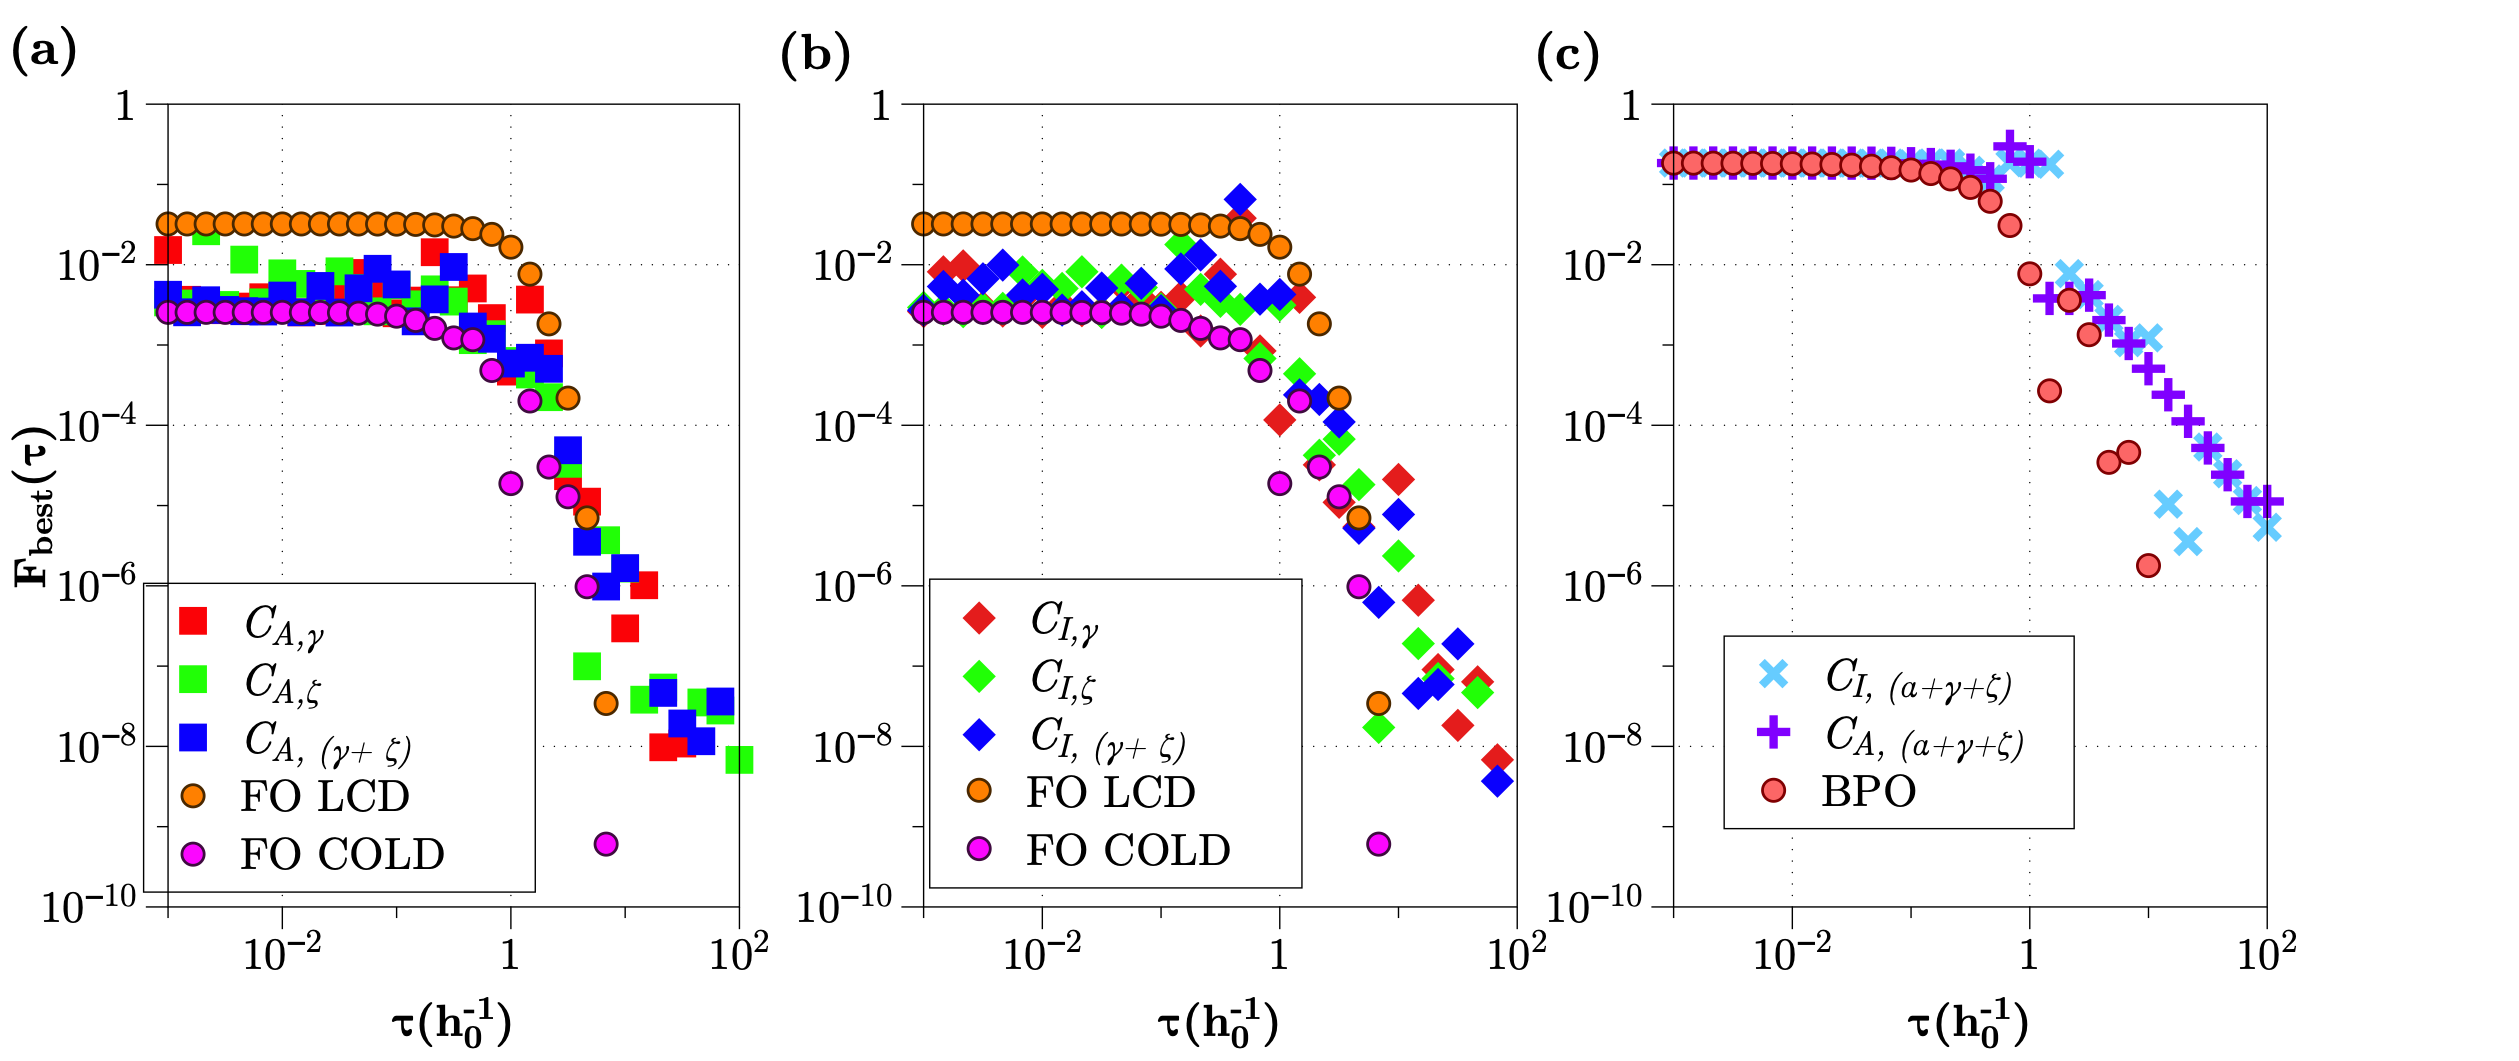
\includegraphics[width=\linewidth]{images/twospin_HO_scatter.png} \caption[Two-spin annealing plots of fidelity versus driving time when minimising different orders of LCD.]{Two-spin annealing plots of fidelity versus driving time when optimising using different cost functions. In (a)-(b), we show the results for \acrref{FO} \acrref{LCD} (orange circles) and \acrref{FO} \acrref{COLD} (pink circles) from Fig.~\ref{fig:twospin_fidelities} for comparison. We do the same in (c) for \acrref{BPO} (red circles). Then, in (a) we plot the resulting final state fidelities at different driving times $\tau$ obtained when applying \acrref{FO} \acrref{COLD} to control Hamiltonians from Eq.~\eqref{eq:COLD_twospin_controlH} with parameters optimised using the maximum amplitude cost function $C_{\rm A}$. The results are shown when optimising for $\gamma$ coefficients (red squares, $C_{\rm A, \gamma}$), $\zeta$ coefficients (green squares, $C_{\rm A, \zeta}$) and their sum (blue squares, $C_{\rm A, (\gamma + \zeta)}$). The same is done in (b) for the integral cost function $C_{\rm I}$, where we plot results in the case of optimising $\gamma$ coefficients (red diamonds, $C_{\rm I, \gamma}$), $\zeta$ coefficients (green diamonds, $C_{\rm I, \zeta}$) and their sum (blue diamonds, $C_{\rm I, (\gamma + \zeta)}$). In (c), we plot the resulting final state fidelities when \acrref{BPO} is applied with a control pulse optimised using $C_{\rm I, (\alpha + \gamma + \zeta)}$ (light blue crosses) and $C_{\rm A, (\alpha + \gamma + \zeta)}$ (purple pluses). In all cases, we use $N_k = 1$. The optimisation is done 10 times for each data point with the best final fidelity plotted. We use the Powell optimisation method from Sec.~\ref{sec:3.1.3.2_Powell} for the minimisation.}\label{fig:twospin_scatter}
\end{figure}


We know that applying the exact \acrref{CD} pulse made up of all of the \acrref{FO} and \acrref{SO} \acrref{LCD} terms returns unit fidelity regardless of driving time or any optimisable parameters, as shown in Fig.~\ref{fig:twospin_fidelities}. We also found, plotted in the same Figure, that applying \acrref{FO} \acrref{LCD} to the problem without any control pulse performed worse than applying \acrref{COLD} with \acrref{FO} terms, where a control pulse is included and the control parameters are optimised for final state fidelity. In this case, we will use a series of cost functions constructed in a similar manner to Eq.~\eqref{eq:COLD_costfunc_integral} and Eq.~\eqref{eq:COLD_costfunc_maximum} in order to optimise the \acrref{COLD} control pulse without computing the final state fidelity until after the optimisation is done, in order to check how well the optimisation has performed. First, we define the cost functions which use the magnitudes of the coefficient integrals as:
 \begin{equation}\label{eq:twospin_costfunc_int}
    \begin{aligned}
        C_{\rm I, \gamma}(\tau, \betabb) &= \int_{0}^{\tau} dt^{\prime} |\gamma(\lambda(t^{\prime}), \hbb, \betabb)|,\\
        C_{\rm I, \zeta}(\tau, \betabb) &= \int_{0}^{\tau} dt^{\prime} |\zeta(\lambda(t^{\prime}), \hbb, \betabb)|,\\
        C_{\rm I, (\gamma + \zeta))}(\tau, \betabb) &= \int_{0}^{\tau} dt^{\prime} \left(|\gamma(\lambda(t^{\prime}), \hbb, \betabb)| + |\zeta(\lambda(t^{\prime}), \hbb, \betabb)|\right), \\
        C_{\rm I, (\alpha + \gamma + \zeta))}(\tau, \betabb) &= \int_{0}^{\tau} dt^{\prime} \left(|\alpha(\lambda(t^{\prime}), \hbb, \betabb)| + |\gamma(\lambda(t^{\prime}), \hbb, \betabb)| + |\zeta(\lambda(t^{\prime}), \hbb, \betabb)|\right),
    \end{aligned}
\end{equation}
where the subscript $I$ denotes an integral-based cost function and the letters $\gamma$ and $\zeta$ simply refer to which pulse coefficient is being minimised for the optimisation process. We then do the same for the maximum amplitude of the pulses, using the subscript $A$ to denote `amplitude':
\begin{equation}\label{eq:twospin_costfunc_amp}
    \begin{aligned}
        C_{\rm A, \gamma}(\tau, \betabb) &= \max_{t^{\prime} \in [0,\tau]} | \gamma(\lambda(t^{\prime}), \hbb, \betabb)|,\\
        C_{\rm A, \zeta}(\tau, \betabb) &= \max_{t^{\prime} \in [0,\tau]} | \zeta(\lambda(t^{\prime}), \hbb, \betabb)|,\\
        C_{\rm A, (\gamma + \zeta)}(\tau, \betabb) &= \max_{t^{\prime} \in [0,\tau]} \left(| \gamma(\lambda(t^{\prime}), \hbb, \betabb)| + |\zeta(\lambda(t^{\prime}), \hbb, \betabb)| \right),\\
        C_{\rm A, (\alpha + \gamma + \zeta)}(\tau, \betabb) &= \max_{t^{\prime} \in [0,\tau]} \left(| \alpha(\lambda(t^{\prime}), \hbb, \betabb)| + |\gamma(\lambda(t^{\prime}), \hbb, \betabb)| + |\zeta(\lambda(t^{\prime}), \hbb, \betabb)| \right),
    \end{aligned}
\end{equation}
which are used to optimise the parameters $\betabb$ by minimising the maximum amplitude of the given \acrref{LCD} coefficients.

The results of optimising for the \acrref{SO} \acrref{LCD} coefficients $\gamma$ and $\zeta$ are plotted in Fig.~\ref{fig:twospin_scatter}(a) and (b). In (a) we show the results of using $C_{\rm A, \gamma}$, $C_{\rm A, \zeta}$ and $C_{\rm A, (\gamma + \zeta)}$ as cost functions for optimising a \acrref{FO} \acrref{COLD} pulse, with \acrref{FO} \acrref{LCD} and \acrref{FO} \acrref{COLD} (optimised using fidelity) from Fig.~\ref{fig:twospin_fidelities} plotted for comparison. We do the same for the respective integral cost functions in (b). The results indicate that while optimising for final state fidelity, not unexpectedly, shows better final state fidelities when \acrref{COLD} is applied, the amplitude and integral cost functions still generally perform better in producing a state close to the target ground state than a naive application of \acrref{FO} \acrref{LCD} with no optimal control. This is a positive result, as it implies that there is a correlation between properties of the \acrref{LCD} coefficients and the final state fidelity in designing optimal control pulses. This is exemplified further in plot (c) of the figure, where we optimise the pulse for a case when no \acrref{LCD} is applied, using a minimisation of the exact \acrref{CD} pulse comprised of all three \acrref{LCD} coefficients. At short evolution times, the optimisation performs as well as the fidelity cost function, while at longer times it begins to lag a little, with a few outliers appearing potentially due to local minima in the cost function landscape. This is to be expected, as minimisation of the exact \acrref{CD} pulse should be equivalent to the minimisation of non-adiabatic effects experienced by the system, and at very short driving times these will probably dominate the loss of final stat fidelity, while at longer times there may be several paths in parameter space that are similarly effective. 

\begin{figure}[t!]
    \centering
    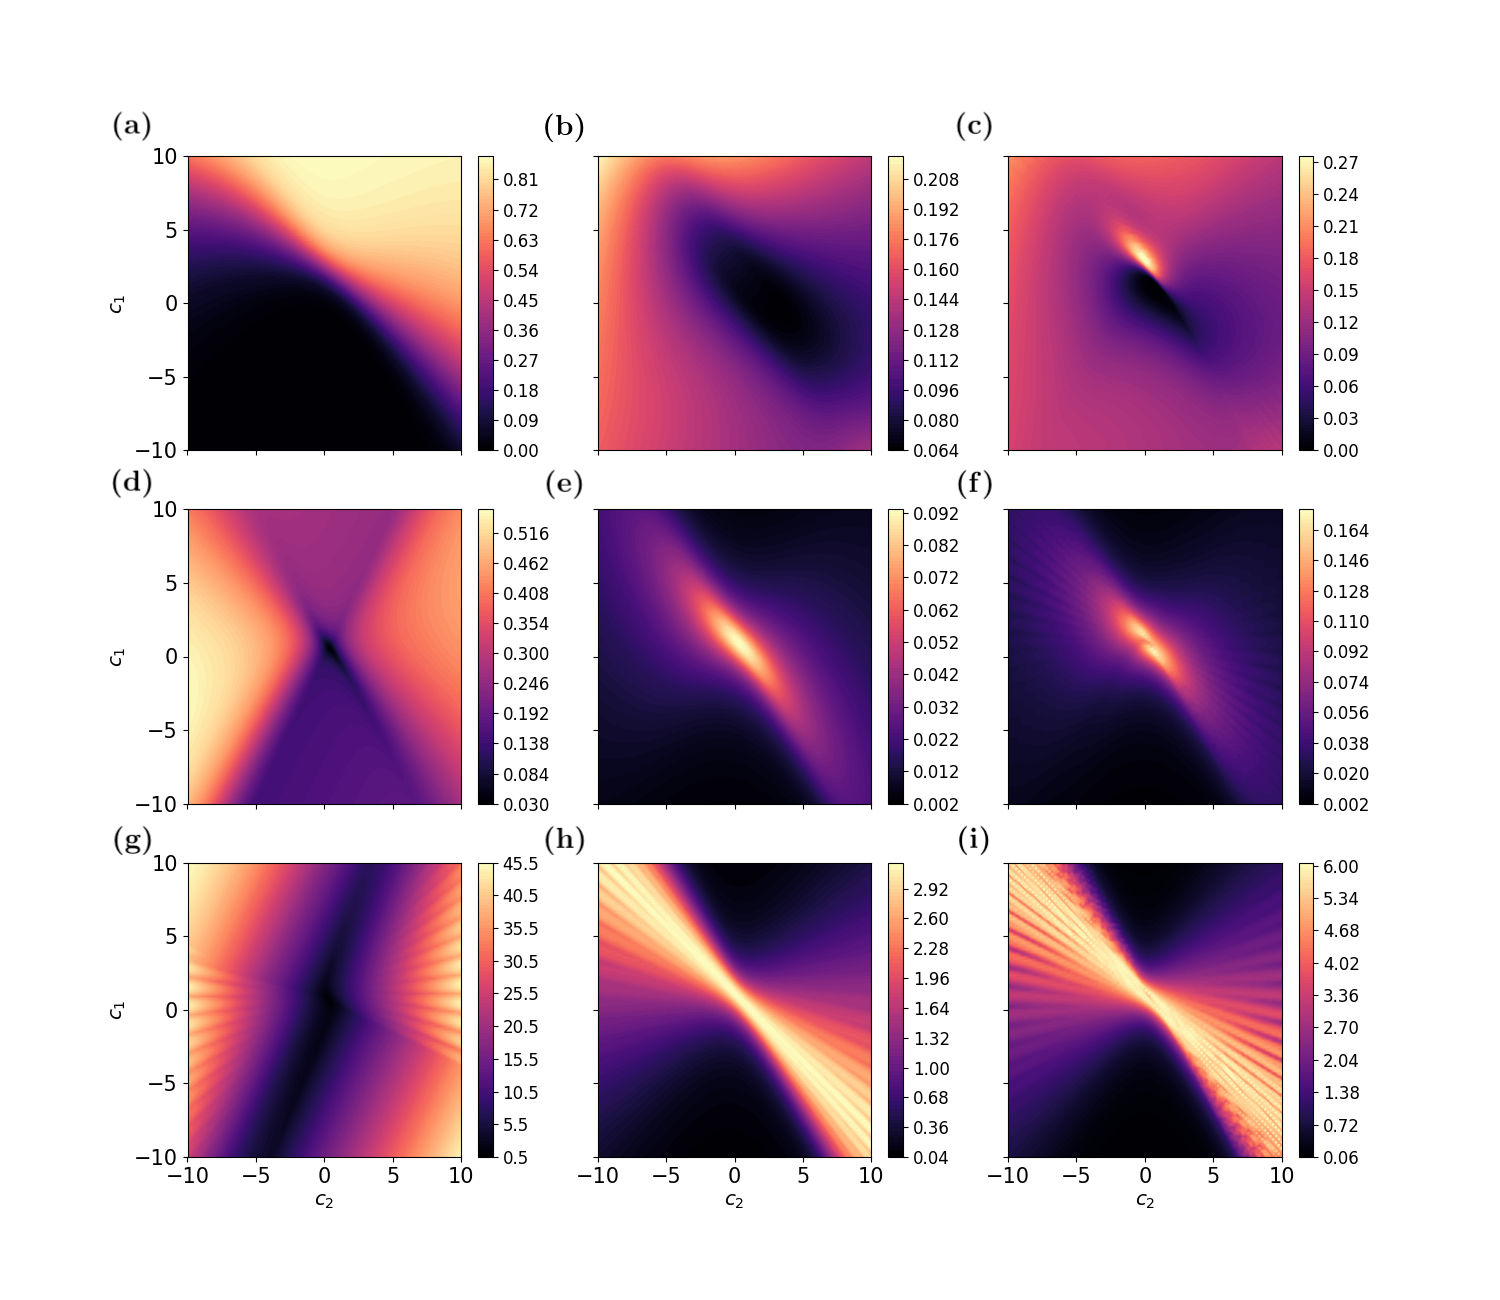
\includegraphics[width=\linewidth]{images/two_spin_contours.png} \caption[Two-spin annealing contour plots for final state fidelity and AGP cost function values.]{Contour plots of fidelity and \acrref{AGP} cost function landscapes for two parameters $c_1, c_2 \in [-10, 10]$ for two spin annealing, as discussed in the text. All plots are for total evolution time $\tau = 0.1 h_0^{-1}$. (a-c) show plots of fidelity cost function $C_{\rm F}$ values when (a) \acrref{FO} \acrref{COLD} is applied ($\alpha$ terms), (b) \acrref{SO} \acrref{COLD} $\zeta$ terms are applied and (c) both \acrref{SO} \acrref{COLD} terms $\gamma$ and $\zeta$ are applied as discussed in the text. (d-f) show plots of the integral cost function $C_{\rm I}$ values for (d) the coefficient $\alpha$, $C_{\rm I, \alpha}$ (e) the coefficient $\zeta$, $C_{\rm I, \zeta}$ and (f) sum of the coefficients $\gamma$ and $\zeta$, $C_{\rm I, \gamma + \zeta}$. (g-i) do the same for $C_{\rm A}$, where (g) shows a plot of $C_{\rm A, \alpha}$, (h) shows $C_{\rm A, \zeta}$ and (i) is a plot of $C_{\rm A, \gamma + \zeta}$}\label{fig:two_spin_higher_order}
\end{figure}

In order to better understand the relationship between the \acrref{LCD} coefficients and the value of the final state fidelity with respect to the target, in Fig.~\ref{fig:two_spin_higher_order}(a-c) we plot the cost function landscapes for fidelity ($C_{\rm F}$) at $\tau = 0.1h_0^{-1}$ for two parameters $c_1$ and $c-2$ in the range $[-10, 10]$. In (a) we plot the value of $C_{\rm F}$ when \acrref{FO} \acrref{COLD} is applied, which corresponds to the $C_{\rm F}$ landscape for the orange circle plots in Fig.~\ref{fig:twospin_scatter}(a-b). Then, in (b) we plot the values of $C_{\rm F}$ when \acrref{COLD} with only the $\zeta$ terms $\sy_1\sz_2 + \sz_1\sy_2$ is applied. Finally, in (c), we plot $C_{\rm F}$ for  \acrref{COLD} with both of the \acrref{SO} terms $\gamma$ and $\zeta$ applied.  We then do the same for $C_{\rm I, \alpha}$ in (d), $C_{\rm I,\zeta}$ in (e) and $C_{\rm I,(\gamma + \zeta)}$ in (f). This is also done for the respective maximum amplitude cost functions. The $\alpha$ coefficients for (a), (d) and (g) are obtained by solving the coupled equations of Eq.~\eqref{eq:two_spin_coupled_eqs} with $\gamma$ and $\zeta$ set to $0$, while for the plots in (b),(e) and (h) we set $\alpha$ to $0$, and find that the $\gamma$ pulse turns out to be $0$ for all values of $\betabb$ and $\lambda$, hence retaining only values of $\zeta$. In (c),(f) and (i) we solve for the full \acrref{CD} pulse with all coefficients but only plot the \acrref{SO} components. What we find is that while there appears to be some relationship between the maximum and minimum of the \acrref{AGP} cost functions and the final state fidelities, it is not clear cut. Certainly, where the final state fidelity $F(\tau)$ is maximised in (a) (\@i.e.~when the plot shows a minimum value as $C_{\rm F} = 1 - F$), the \acrref{SO} \acrref{LCD} plots (e-f) and (h-i) have small values. However, it appears as though the \acrref{SO} components are also small for values of $c_1$ and $c_2$ which lead to very bad final state fidelities in (a). It is also clear that maximising fidelity for \acrref{FO} \acrref{COLD} is not necessarily equivalent to maximising the \acrref{FO} \acrref{LCD} coefficient. What these plots are intended to illustrate is that while there appears to be some relationship between the various approximations of the \acrref{AGP} and the final state fidelity of the system when \acrref{COLD} of various orders is applied, this relationship need not be clear cut.

We note that there is no contour plot for $C_{\rm F}$ in the case of \acrref{BPO} nor plots of the integral or amplitude functions for the exact \acrref{CD} pulse comprised of all of the \acrref{LCD} coefficients and that is because the optimal parameter values of $c_1$ and $c_2$ were very large (of the order of $1\times10^3 h_0^{-1}$) and varied in the results of Fig.~\ref{fig:twospin_scatter}(c), making it difficult to capture the relevant cost function landscapes visually. The fact that the \acrref{COLD} optimal control pulses require quite low amplitudes even at short driving times could, in fact, also be considered an advantage of the method.

While in this simple example it may be more favourable to implement the fidelity cost function $C_{\rm F}$ given that for two spins it is reasonably efficient to compute the state evolution, in more complex systems this is no longer the case. Iterative optimisation procedures like Powell's method (Sec.~\ref{sec:3.1.3.2_Powell}), which we have been using, may require hundreds or thousands of cost function evaluations for a single optimisation procedure. The fact that we get results which are comparable to $C_{\rm F}$ while using a set of cost functions which become exponentially more efficient to implement as the system size grows is something that can become very useful in such more complex cases.

\section{Return to the Ising spin chain}\label{sec:7.2_ising_ho_lcd}

As in the previous section, here we revisit a system that was already explored in the previous chapter: the Ising spin chain of Sec.~\ref{sec:5.2_Ising_chain}. As in the two-spin case, we are interested in retaining the same parameters as those explored for \acrref{COLD} with the fidelity cost function, changing only the optimisation landscape via the integral and amplitude cost functions outlined in Eq.~\eqref{eq:twospin_costfunc_int} and Eq.~\eqref{eq:twospin_costfunc_amp} respectively. Thus, we use the same bare Hamiltonian and parameters (Eq.~\eqref{eq:ising_hamiltonian}) along with the Powell optimal control pulse from Eq.~\eqref{eq:ising_chain_BPO_H}, parameterised by the control functions $\beta_k \in \betabb$ and by constant control parameters $c_k$. The \acrref{FO} \acrref{LCD} ansatz is still the same as in Eq.~\eqref{eq:ising_fo_agp}, which is a set of local $\sy$ operators on each spin and the \acrref{SO} operators are taken to be all of the nearest neighbour, two-body Pauli terms on $N$ spins, expressed as
\begin{equation}\label{eq:ising_so_lcd_terms}
    \begin{aligned}
        \approxAGP^{(2)}(\betabb, \hbb, \lambda) = & \sum_j^{N-1} \gamma(\betabb, \hbb, \lambda) (\sx_j\sy_{j+1} + \sy_j\sx_{j+1}) \\
        &+ \sum_j^{N-1} \zeta(\betabb, \hbb, \lambda) (\sz_j\sy_{j+1} + \sy_j\sz_{j+1}),
    \end{aligned}
\end{equation}
where $\gamma$ and $\zeta$ are the \acrref{SO} \acrref{LCD} coefficients as in the previous example. In this section we use the same integral and amplitude cost functions as in Eq.~\eqref{eq:twospin_costfunc_int} and Eq.~\eqref{eq:twospin_costfunc_amp}, with the coefficients $\alpha$, $\gamma$ and $\zeta$ as presented above. These can be solved for by using the results presented in Appendix~\ref{app:arbitrary_ising_derivation}, as discussed in Sec.~\ref{sec:5.2_Ising_chain}.

The main difference between the two spin example and this one, in particular when considering using \acrref{AGP} constructed cost functions, is that for increasing spin chain lengths we can no longer expect to have access to the exact \acrref{CD} pulse, as the non-adiabatic effects may become delocalised quickly throughout the chain. Even if the effects of the delocalised \acrref{AGP} operators are small, they are not necessarily guaranteed to be non-zero. Thus, we are now operating in a setting where we might not have all of the information about the non-adiabatic effects on the system and must instead contend with \acrref{LCD} approximations of the exact counterdiabatic pulse explicitly.
\begin{figure}[t]
    \centering
    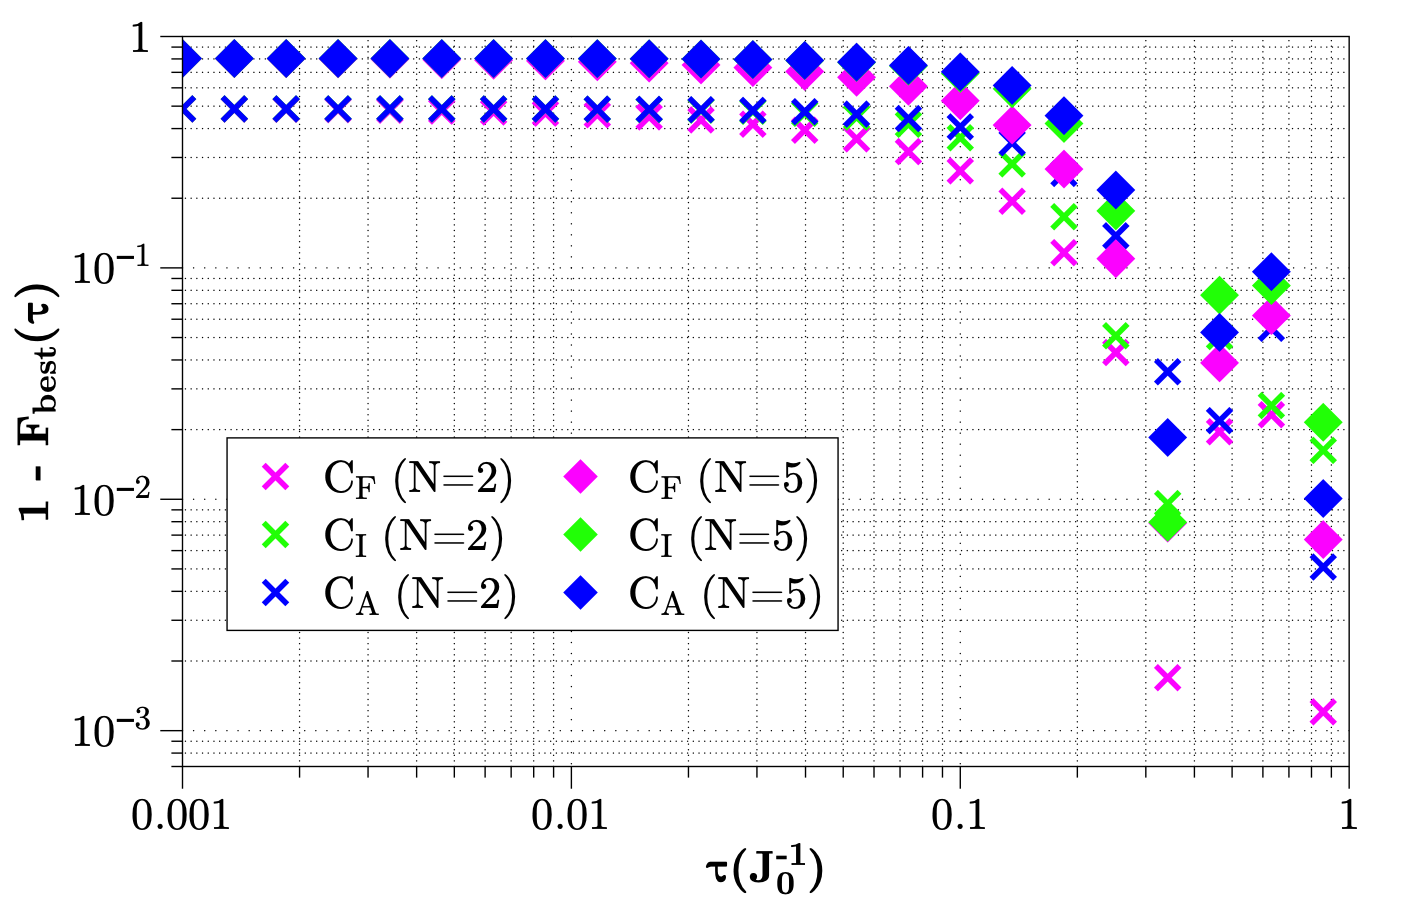
\includegraphics[width=0.8\linewidth]{images/No_cd_higher_order.png} \caption[Plot of final state fidelity for the Ising spin chain for different cost functions and no counterdiabatic component in the implementation.]{Plot of final state fidelities obtained when optimising for the fidelity cost function $C_{\rm F}$ (pink), the integral cost function for \acrref{FO} and \acrref{SO} \acrref{LCD} pulses $C_{\rm I, (\alpha + \gamma + \zeta)}$ (green) as well as the maximum amplitude cost function $C_{\rm A, (\alpha + \gamma + \zeta)}$ (blue). We plot results for two spins (crosses) and five spins (diamonds), optimising separately for both. Results are plotted for $N_k = 1$ and different total driving times $\tau$. Optimisation is performed 10 times for each data point and the lowest obtained value for the cost function is used to compute the fidelity in the case of $C_{\rm A}$ and $C_{\rm I}$.}\label{fig:ising_nocd_higher_order}
\end{figure}

With this in mind, the first thing we explore is whether or not we can use the \acrref{FO} and \acrref{SO} \acrref{LCD} coefficients in the same vein as in Fig.~\ref{fig:twospin_scatter}(c) to optimise the \acrref{BPO} pulse. We plot the results in Fig.~\ref{fig:ising_nocd_higher_order} for the cases of $N=2$ spins and $N=5$ spins, using $C_{\rm F}$, $C_{\rm A, (\alpha + \gamma +\zeta)}$ and $C_{\rm I, (\alpha + \gamma +\zeta)}$. We expect that in the two-spin case we will get a similar result as in Fig.~\ref{fig:twospin_scatter}(c), given that we should be minimising the exact \acrref{CD} pulse in the case of two spins when using both \acrref{FO} and \acrref{SO} in the cost function and this appears to be the case: at short evolution times, the results of the final state fidelity match up regardless of which cost function is used, while at longer times $C_{\rm F}$ begins to perform better, although all cost functions show a similar pattern in final state fidelity scaling with $\tau$. However, in the five spin case, we do not have an explicit reason to expect a similar behaviour unless higher order \acrref{LCD} does not play a big part in the non-adiabatic effects experienced by the system. It turns out, in fact, that this is the case: the behaviour for five spins is comparable to that of two spins: at short times the cost functions are equally as effective, with differences appearing only at longer times. 

\begin{figure}[t!]
    \centering
    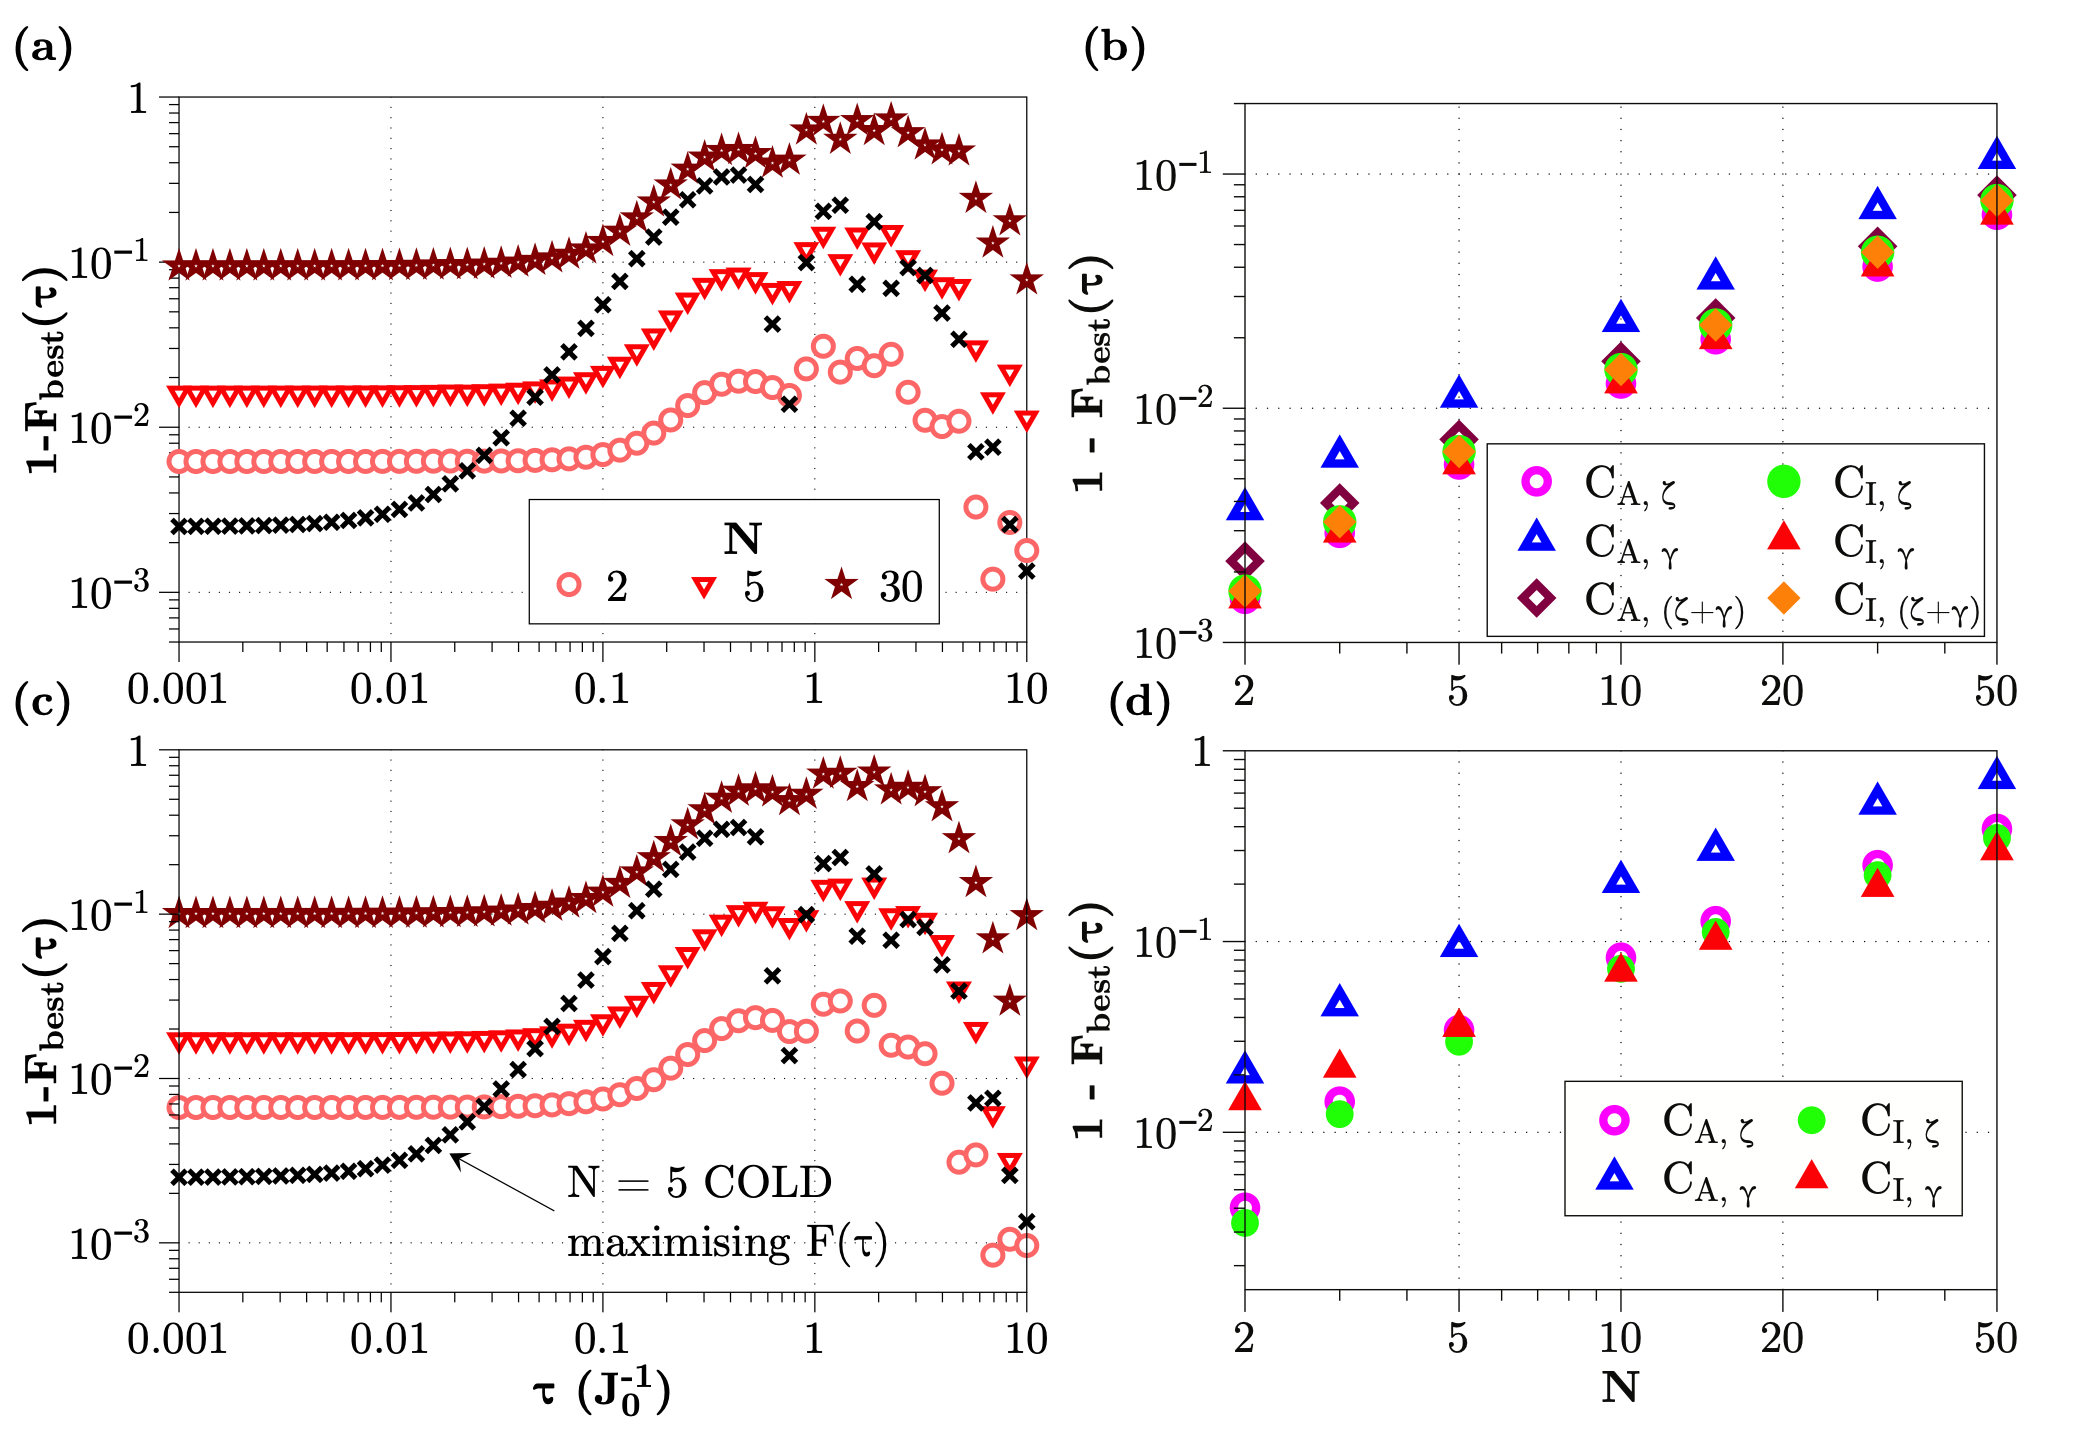
\includegraphics[width=\linewidth]{images/ising_max_int_plots.png} \caption[Plot of final state fidelity for the Ising spin chain for different cost functions with LCD applied.]{Final state fidelities when control parameters are optimised via integral and amplitude cost functions of the \acrref{SO} \acrref{LCD} coefficients for the Ising spin chain with \acrref{FO} \acrref{COLD} applied to the system. In (a) we plot the results obtained when using the integral cost function $C_{\rm I, (\zeta)}$ and in (c) we do the same in the case of maximum amplitude $C_{\rm A, (\zeta)}$ for Ising chains of lengths $N = 2$ (pink circles), $N = 5$ (red inverted triangles) and $N=30$ (dark red stars). We also plot results for \acrref{COLD} optimisation with $C_{\rm F}$ in the case of $N=5$ spins from Fig.~\ref{fig:ising_unconstrained}(a) for comparison (black crosses). We investigate how the different cost functions perform for evolution time $\tau = 0.1J_0^{-1}$ for different system sizes $N$ in the case where (b) \acrref{FO} \acrref{COLD} is applied to the system while minimising a \acrref{SO} component and (d) when applying both \acrref{FO} terms and one of the \acrref{SO} terms. For example, in (d), the pink circles are the result of implementing \acrref{COLD} with \acrref{FO} local $\sy$ terms and $\gamma$ terms $\sx\sy$, $\sy\sx$ while minimising the maximal amplitudes of the $\zeta$ terms $\sz\sy$, $\sy\sz$. For system sizes above $N=10$ we used ITensor\cite{fishman_itensor_2022} MPS calculations which were converged with a truncation level of $10^{-14}$ per time step. at each site reaching a maximum bond dimension of $D = 4$. In all cases, a single optimisable parameter is used ($N_k = 1$) and the best optimisation out of 50 (lowest cost function value for each cost function) is used. Reprinted with permission from \cite{cepaite_counterdiabatic_2023}. Copyright 2023, American Physical Society.}\label{fig:ising_minimising_ho_mainplot}
\end{figure}

The other case that we can explore, then, to improve our results, is to see if we could implement \acrref{FO} or partial \acrref{SO} \acrref{COLD} while minimising the other \acrref{LCD} term coefficients. This is presented in Fig.~\ref{fig:ising_minimising_ho_mainplot}, where in (a-b) we implement \acrref{COLD} with \acrref{FO} \acrref{LCD} coefficients while minimising the integral cost function $C_{\rm I, (\zeta)}$ in (a) and the amplitude cost function $C_{\rm A, (\zeta)}$ in (c), both for system sizes of $N = 2, 5, 30$. We also plot the results from Fig.~\ref{fig:ising_unconstrained}(a) which show results when optimising \acrref{COLD} using the final state fidelity cost function $C_{\rm F}$ in the case of $N = 5$ spins for fidelity. What we find is a consistent pattern in the behaviour of the final state fidelity when using either of the two cost functions, with consistently stable final fidelities at shorter driving times and, surprisingly, better final fidelities at longer driving times, at least in the $N=5$ case. We might attribute this to different cost function landscapes due to the different cost functions, which might have more or less optimal minima within reach for a local optimiser like Powell's method (Sec.~\ref{sec:3.1.3.2_Powell}). Regardless, what we do find is that we can get final state fidelities consistently above $90\%$ for a system of $N=30$ spins while using an exponentially more efficient cost function for optimisation. While we use tensor network methods to compute the fidelities of chains with $N=10$ spins and above in all cases, these approaches are still orders of magnitude slower at calculating a single iteration of the $C_{\rm F}$ cost function than in the case of  either of the integral or amplitude cost functions used for the optimisation. We find that this trend is consistent, if slightly shifted depending on which \acrref{AGP}-based cost function is used in plot (b) of Fig.~\ref{fig:ising_minimising_ho_mainplot}, and that this trend is consistent when minimising one of the \acrref{SO} coefficients and implementing the other along with the \acrref{FO} terms, at least at relatively short driving times of $\tau = 0.1J_0^{-1}$.

All of these results are not conclusive proof for the advantage of using the integral or amplitude cost functions in place of $C_{\rm F}$, especially if the \acrref{LCD} terms are highly local with respect to the full system size. However, the results presented do indicate a potential advantage, especially in the case of larger systems, of using knowledge about the approximate \acrref{AGP} operator in an optimisation procedure of the control Hamiltonian, assuming the wavefunction of the state is prohibitively difficult to access. In doing so, it is possible to sacrifice some amount of effectiveness for a large gain in efficiency and, possibly, this kind of approach could be used in cases where fidelities are simply not a tractable option in the case of numerical optimisation.

\section{GHZ states and frustrated spins}\label{sec:7.3_ghz_ho}

Finally, we return to the GHZ state preparation scheme from Sec.~\ref{sec:6.4_ghz_states}. Thus far, both in the two-spin case and in the Ising spin chain case we have seen some evidence for advantage when it comes to using \acrref{AGP}-informed cost functions to optimise the control parameters with respect to the final state fidelity. While we have shown that optimising using the fidelity cost function $C_{\rm F}$ generally guarantees better results, it is also far less efficient for larger systems. Using the integral cost function $C_{\rm I}$ or the amplitude cost function $C_{\rm A}$ may not be as effective, but it is far more efficient and can be used to obtain good results for both \acrref{COLD} and optimal control pulses with no \acrref{CD} added to them. In this case, we will explore an example of a system and control pulse combination for which this option may not be viable, at least given the parameters we are working with.

We will set up the problem in the same way as in Sec.~\ref{sec:6.4_ghz_states}, with the bare Hamiltonian from Eq.~\eqref{eq:ghz_hamiltonian}, as well as a \acrref{GRAPE} control pulse as given by Eq.~\eqref{eq:ghz_control} and the surrounding description. In this case, from Sec.~\ref{sec:6.4.1_t3} we recall that we already attempted implementing a different cost function to $C_{\rm F}$, the aim of which was to maximise a measure of tripartite entanglement in the three spin case: $C_{T_3}$ from Eq.~\eqref{eq:tangle_costfunc}. We will return to both the fidelity and the tangle as measures of success for the final state and thus we will be looking solely at the $N=3$ spin example, both as the simplest possible example to test out new cost functions on and due to the fact that we have a non-trivial tripartite entanglement metric like the three-tangle available.

\begin{figure}[t!]
    \centering
    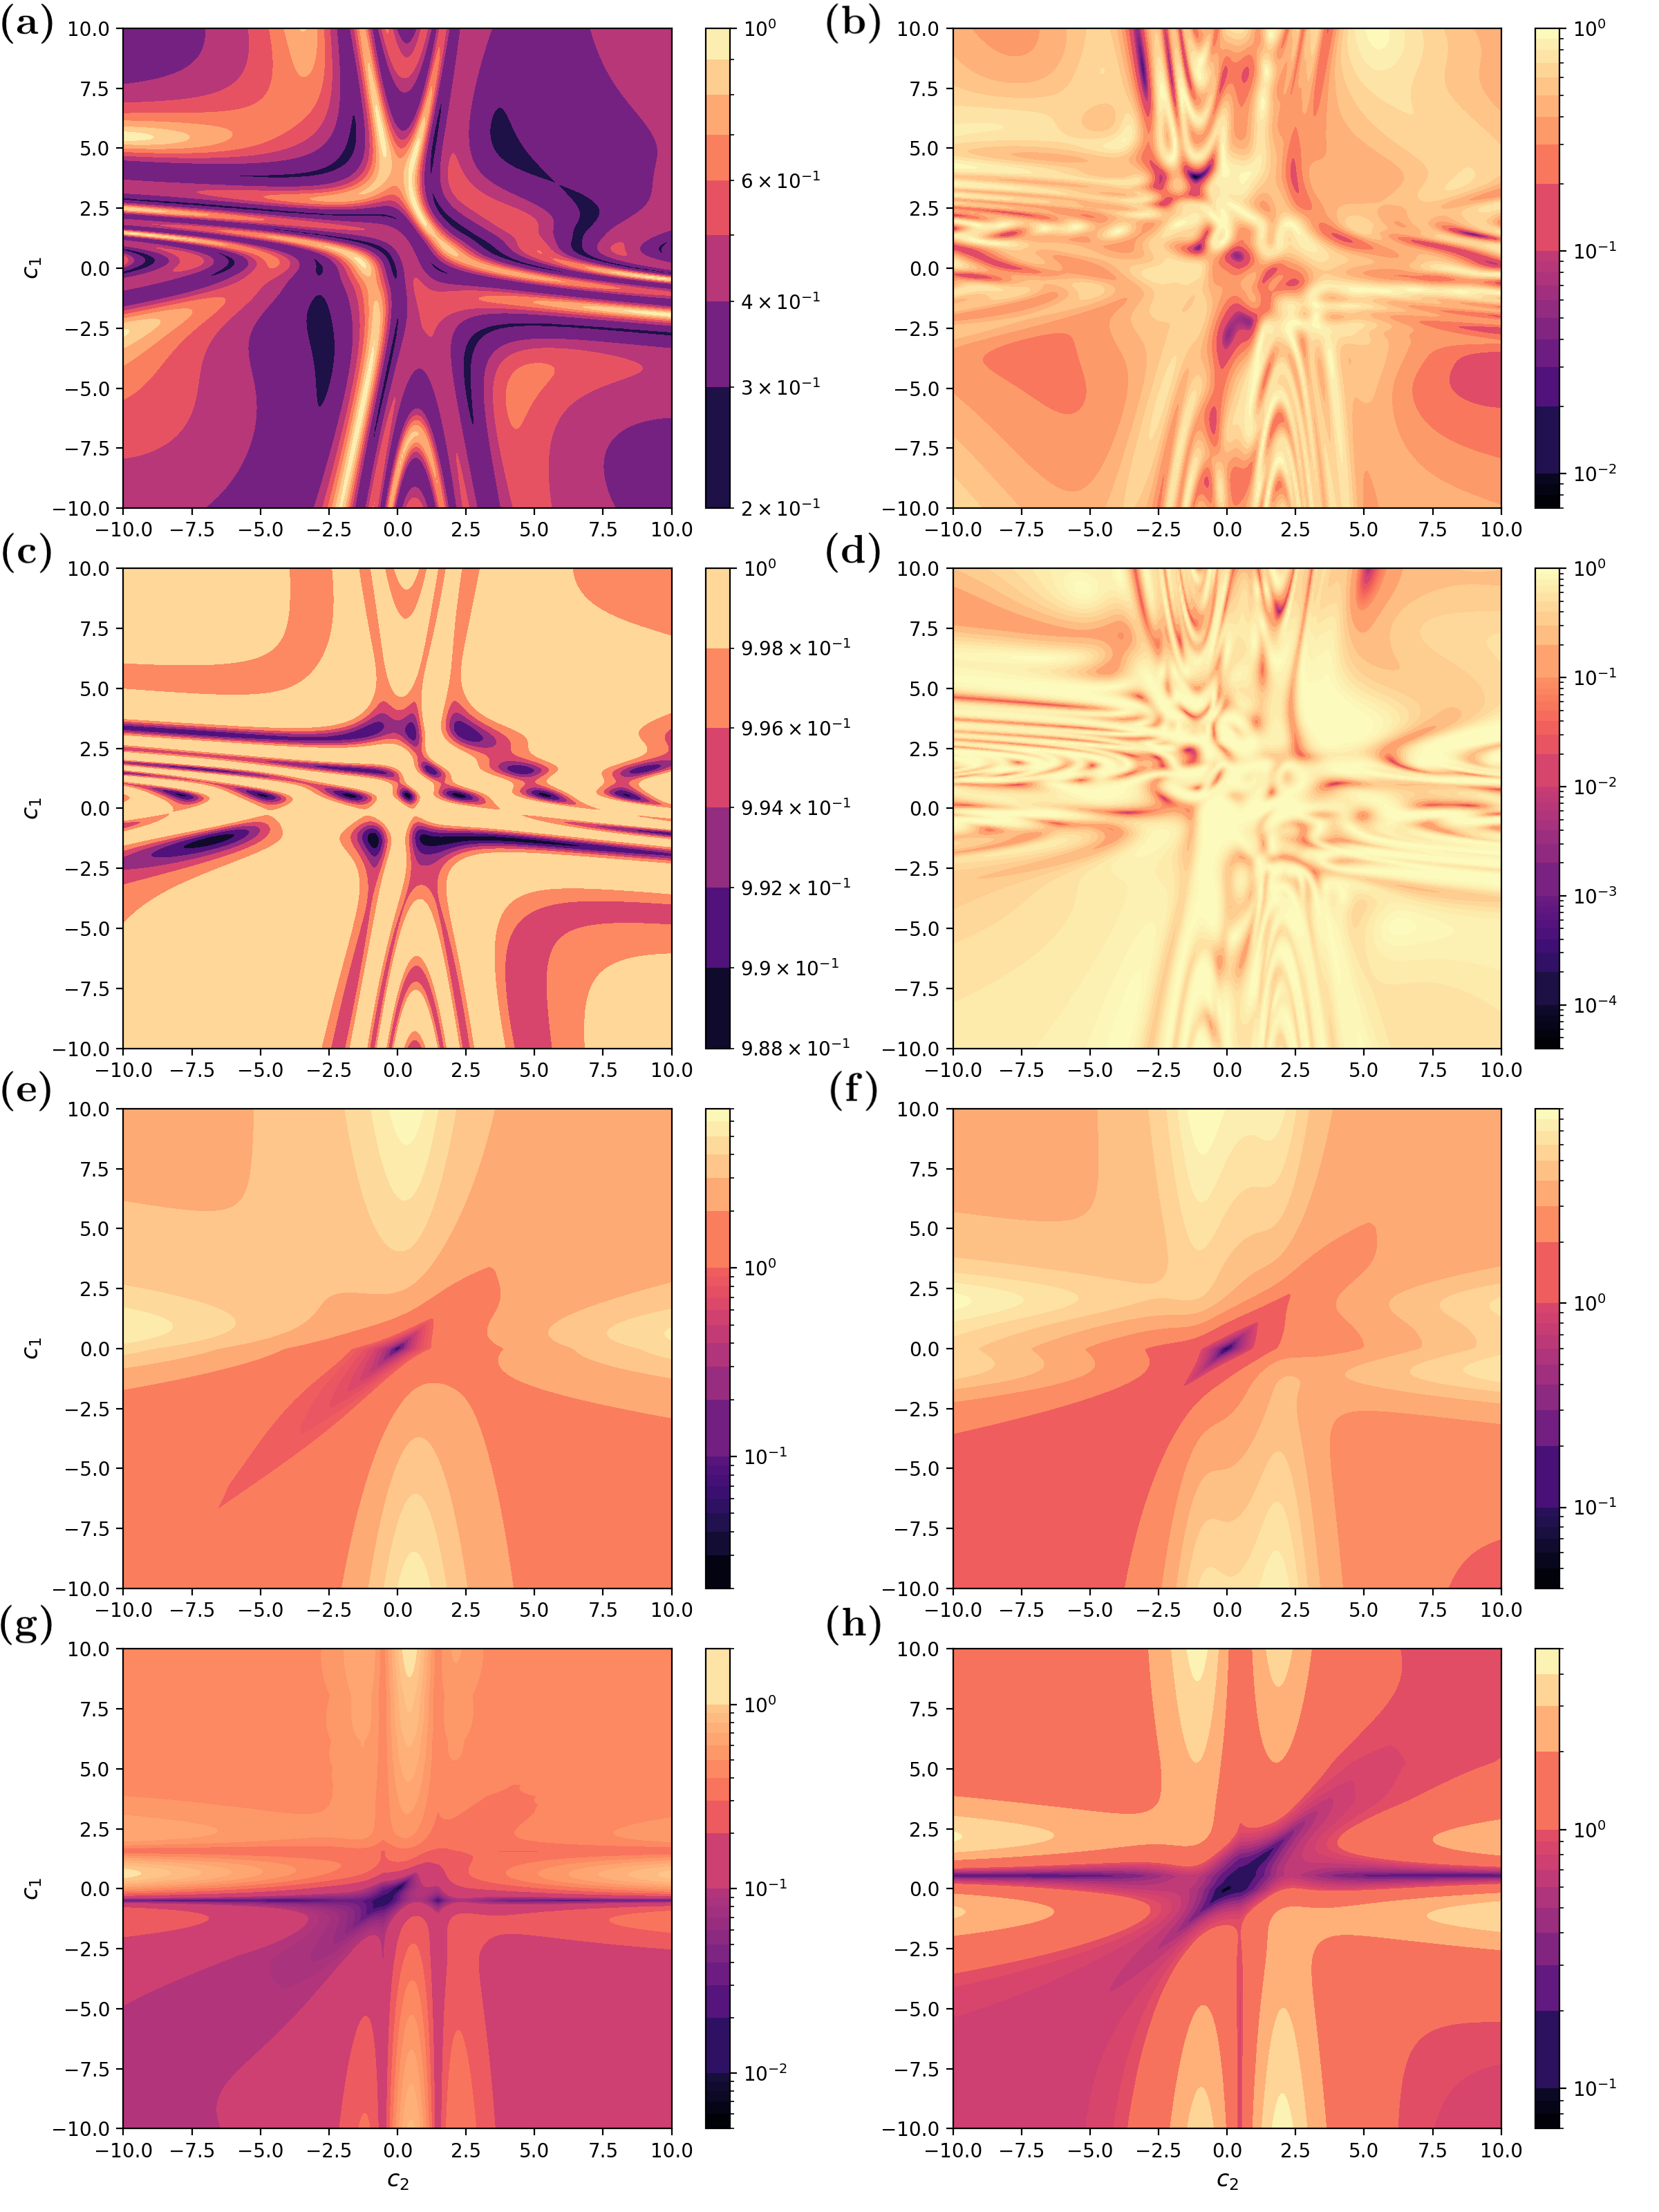
\includegraphics[width=0.75\linewidth]{images/ghz_contour_integrals.png} \caption[Contour plots of cost function landscapes for GHZ state preparation in frustrated spin systems (integral cost function).]{Contour plots at $\tau = 0.1 J_0^{-1}$ of different cost function values for GHZ state preparation for parameters $c_1, c_2 \in [-10,10]$ and a \acrref{GRAPE} control pulse. In (a) and (b) we plot $C_{\rm F}$ in the cases where \acrref{FO} and \acrref{SO} \acrref{COLD} is applied respectively. Then, in (c-d) we do the same for $C_{T_3}$, with \acrref{FO} \acrref{COLD} plotted in (c) and \acrref{SO} \acrref{COLD} plotted in (d). (e-h) are then plots of the integral cost function $C_{\rm I}$ values for the same range of parameters. In (e) we plot $C_{\rm I, \alpha^{(1)}}$ when only \acrref{FO} \acrref{LCD} is considered, while in (f) we plot $C_{\rm I, \alpha^{(2)}}$ as described in the text. Then in (g) we plot $C_{\rm I, \gamma}$ and in (h) we plot $C_{\rm I, \zeta}$, corresponding to the \acrref{SO} terms. Note that each plot has its own colour bar, as the colour encodings and the value scaling in each plot is quite different.}\label{fig:ghz_contours}
\end{figure}

The \acrref{FO} \acrref{LCD} terms are defined as previously to be local $\sy$ operators scaled by the coefficient $\alpha(\betabb, \hbb, \lambda)$, while the \acrref{SO} terms are those presented in Eq.~\eqref{eq:ghz_so_lcd}. We will differentiate here between solving for $\alpha$ when only the \acrref{FO} terms are in the \acrref{LCD} ansatz, denoting this case as $\alpha^{(1)}$ and solving for all of the three coefficients $\alpha$, $\gamma$ and $\zeta$ as a combined \acrref{FO} and \acrref{SO} ansatz by using the coupled set of equations presented in Appendix~\ref{app:arbitrary_ising_derivation}, wherein we will refer to the \acrref{FO} coefficient as $\alpha^{(2)}$ instead.

In Fig.~\ref{fig:ghz_contours} we plot the cost function landscapes for $C_{\rm F}$ (a-b), $C_{T_3}$ (c-d) and several integral cost functions $C_{\rm I}$ in (e-h) for a total driving time of $\tau = 0.1J_0^{-1}$ (the results for the maximal amplitude cost functions can be found in Appendix~\ref{app:higher_order_AGP}). The first thing that one might notice when looking at the plots is that while there appears to be some qualitative relationship between the different cost function landscapes, it is certainly not the case that there is a clear overlap between the minimum or maximum values of the integral cost functions and the highest fidelities (lowest values in the contour plot, as $C_{\rm F} = 1 - F$). This is a fact that holds true in the case of the maximal amplitude cost functions in Appendix~\ref{app:higher_order_AGP} too. The $C_{\rm F}$ and $C_{T_3}$ landscapes are highly non-convex, with multiple local minima close to each other, something that is may be a consequence of the \acrref{GRAPE} cost function and the very small number of parameters, as this translates to very sudden piecewise shifts in the control pulse (see discussion in Sec.~\ref{sec:4.2_COLD_QOCT}). This may also be a consequence of the degenerate nature of the ground state. It is possible, that the reason there is such a disparity between the final state fidelity and the scale of the \acrref{LCD} coefficients is the small number of parameters in the \acrref{GRAPE} function, but attempts to optimise the \acrref{GRAPE} control pulse with parameter numbers up to $N_k = 12$ using dual-annealing (Sec.~\ref{sec:3.1.3.3_dual_annealing}) with $C_{\rm I}$- and $C_{\rm A}$-type cost functions as in Fig.~\ref{fig:ising_minimising_ho_mainplot} or Fig.~\ref{fig:ising_nocd_higher_order} results in the system barely moving out of its initial state regardless of driving time (not plotted). This is certainly an indication that in a more complex regime with a degenerate ground state where the target is entanglement generation, the \acrref{AGP} cost function approach might not work, or at least needs to be investigated further. Perhaps, as we hope to show in future work \cite{lawrence_numerical_2023}, higher orders of the \acrref{LCD} are required in order to capture the non-adiabatic effects associated with entanglement creation.

